\section{Background Information \& Research}
This sections look at some software systems that are already attempting to solve the problem identified in this dissertation, as well as discussing some of the different technologies considered for the implementation of this project.

\subsection{Existing Systems}
\label{sec:existing-systems}
As mentioned in section \ref{sec:intro}, software systems for the distribution and sharing of scenic routes already exist. Each of these systems approaches the problem in a different way, and thus all have their own advantages and disadvantages, which will be discussed here. The aim of this is to determine the best features and the worst features, so they can be incorporate or avoided.

\paragraph{Google's ``My Maps'', \url{https://www.google.com/maps/d}}\ \\
Google's ``My Maps'' service (distinct from ``Google Maps'') is a tool that offers users the ability to plot maps between locations, and save them to their Google accounts. This allows users to quickly access routes they travel frequently, as well share those routes with others (over various social media platforms). The main advantages of this service are that it provides a graphical tool for visualising routes, the ability to add photos and videos to specific waypoints, and, as mentioned above, the ability to share routes via social media. Another interesting feature that is provided is the ability to plot all the point, and generate the route afterwards, rather than generating the route after each point is placed. This is an interesting consideration for a mobile application, because users may wish to save on data (although if users are unaware of this being the reason, it just makes the tool look less responsive).\ \\
\ \\
The key disadvantage of Google's ``My Maps'' is that it is very slow, and there are long periods of loading in-between successive actions. Responsiveness on websites is key, otherwise users are unaware if their actions are having an impact or not. There are also other disadvantages, including the unintuitive and cluttered user interface, the small user base (being a relatively unknown piece of software, dwarfed by the Google Maps service), and that the only way of sharing your routes is to other social media platforms. This last point is particularly important to address for Niceway.to, because it aims is to build a community of users. If they can only share their routes to \textit{other} platforms, the community will have a much smaller chance of thriving. This is why all routes on Niceway.to will be accessible and searchable from within the system itself, and the sharing of routes will simply be a tool to draw more people to the site.

\begin{figure}[!ht]
	\begin{center}
		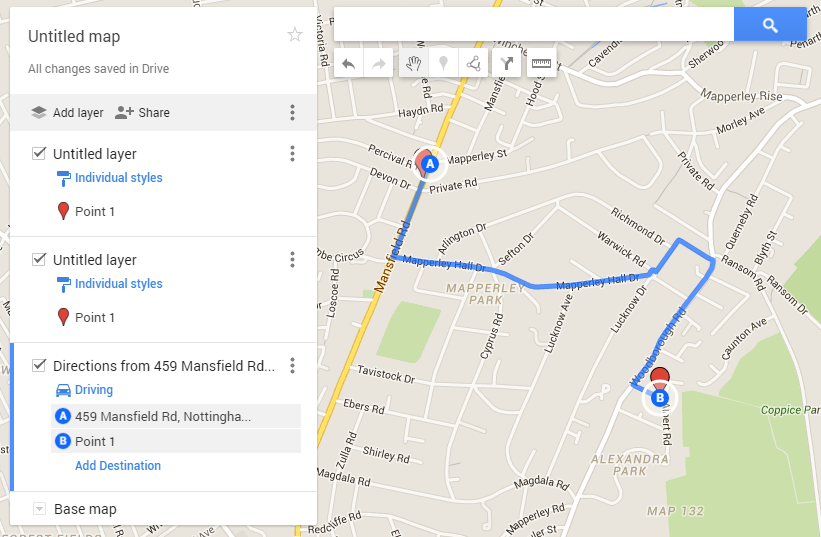
\includegraphics[width=0.66\textwidth]{images/background/gm_rcp.png}
	\end{center}
	\vspace{-6mm}
	\caption{Google's ``My Maps'' route creation/editing feature}
	\vspace{-6mm}
\end{figure}

\newpage 
\paragraph{MyScenicDrives, \url{https://www.myscenicdrives.com}}
\begin{wrapfigure}{r}{0.45\textwidth}
	\vspace{1mm}
	\begin{center}
		\hspace{5mm}
		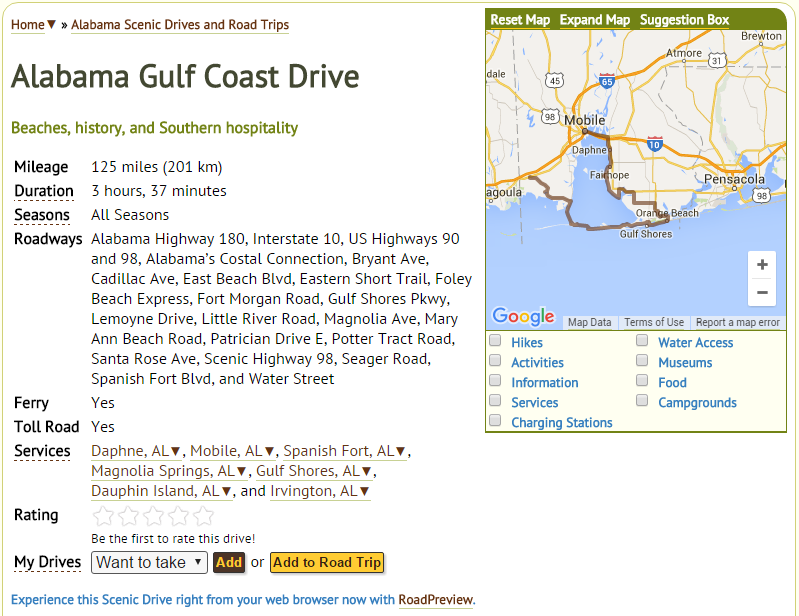
\includegraphics[width=0.45\textwidth]{images/background/msd_rdp.png}
	\end{center}
	\vspace{-6mm}
	\caption{MyScenicDrive's route details}	
	\vspace{-10mm}
\end{wrapfigure}
MyScenicDrives is a website that allows users to search for scenic routes by city, state or zip code (currently the service is only available in the United States), and view extremely detailed information about these routes. This includes a very lengthy explanation of all the things can be seen and done on the journey, interesting facts about the locations visited, all the roads that will be driven on, the best seasons to take the journey during, and even which service stations will be passed. This extremely rich content is the main selling of MyScenicDrives.

\vspace{5mm}
\noindent 
However, no matter how high the quality of this content it, there is still a glaring problem with MyScenicDrives: the quantity of routes. This may be due to the huge amount of information required for a route to be accepted onto the site, but essentially makes the entire application useless. As an example, a search for all routes in the state of Alabama returned a single result. In addition to this, the search functionality itself is very primitive. There is no option for users to select where they wish to start or end their journey, and instead they can only pick a large geographic region. Which would not be suitable for Niceway.to, which aims to provide a way for users to find routes between specific locations.
\ \\
\paragraph{Mad Maps, \url{http://madmaps.net/}}\ \\
The final mapping website that was investigated was Mad Maps, which differed from the others in that it allowed users to purchase physical maps, which they could also view on their mobile phones. One useful feature of the service was the ability to download routes directly to a mobile device, so that the user's Internet connection did not become a limiting factor during a journey. However, it is difficult to ignore the biggest down fall of this service, which was the cost associated with it. All of the maps had a price associated with them, and there was no ability to preview the maps before purchasing. This blind investment could be off putting for many users, as they may be unsure if they will even enjoy the routes provided. Further to this, the mobile application both required an upfront payment to download, as well as containing adverts within it: which seems unjustified when the majority of the Mad Maps applications had very poor reviews.
\begin{wrapfigure}{l}{0.4\textwidth}
	\vspace{-1mm}
	\hspace{5mm}
	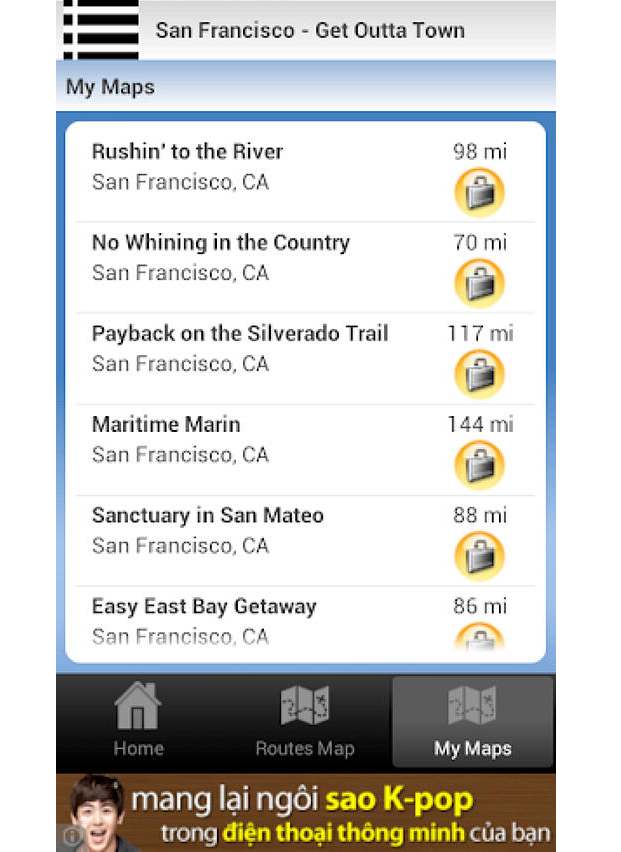
\includegraphics[width=0.35\textwidth]{images/background/mm_rlp.png}
	\centering
	\caption{List of Mad Maps routes}	
	\vspace{-40mm}
\end{wrapfigure}
\ \\
The service works by having a group of ``experts'' compile the maps, and distribute them to the users. This is supposed to instil confidence of their quality, but instead takes out a huge part of travelling, which is the social experience. The only social interaction that users can have with Mad Maps, is the ability to upload photos of waypoints that they have visited, but these will then only be seen by other users that have purchased the route, and would not help to foster the community that Niceway.to is striving for. 

\newpage 
\subsection{Platforms and Tools}
\label{sec:pat}
This section introduces some potential platforms and tools that could have been used in the project, along with justifications for and against them. The system consisted of the back end and server technologies, as well as some user-friendly front end. Tools and frameworks and languages for both of these parts were evaluated to determine which would be the most appropriate. A full list of the final decisions of tools to use, including their justifications, can be found in section \ref{sec:kid}.

\subsubsection{Native Mobile Applications VS Responsive Web Applications}
Before investigating technologies to use, it was important to determine what kind of application was to be developed, as this would radically change the tools required. Ultimately, it was decided that it would be better to build Niceway.to as a responsive web-application, but the advantages and disadvantages of both approaches have been discussed below.

\paragraph{Native Mobile Application}\ \\
Native mobile applications are applications that are downloaded onto a mobile device, and run directly on the hardware. These applications generally have greater exposure, because they are distributed through the application marketplace for the given operating system, and can be reviewed and rated by users. There are several advantages to developing a native mobile application including: the ability to implement multiple pricing models (payment for download, in-application purchases, free with advertisements, or entirely free), after the initial download they can be used without an Internet connection (as data can be downloaded to the phone and accessed later), and the native technology and hardware of the phone can be utilised to provide a better experience for the user.\ \\
\ \\
However, native applications do also have some drawbacks. The most prominent is the number of different operating systems available, which mean that any application created needs to be rewritten multiple times in different languages, to ensure that it can target all devices. This is a huge investment of time and resources, especially as some platforms do not have a large user base (and therefore this effort would potentially be wasted). Native applications must also be downloaded onto the user's device, which requires a commitment from the user, and their on-going desire to keep the application on their phone. Mobile phone users can be fickle, and delete the application at any time for any number of reasons. 

\paragraph{Responsive Web Application}\ \\
A responsive web application is a website that can function both on desktop devices, and mobile devices by scaling the elements on display. They are incredibly versatile because they run in a web browser, which means that they target all possible devices without the need to rewrite the code base in several languages (some tweaks for certain browsers may be required, but this is usually a small amount of work). They are written in the default web languages of HTML, CSS and JavaScript, and the back end can be whichever language the developers are most comfortable with, which makes it very easy for developers of any skill level to work on them. Another advantage of them being hosted on a server online is that it becomes very easy to release updates, because they are instantaneous, and the users do not have to download anything.\\
\ \\
However, the Internet is a large place, and without a centralised place to advertise the application, it is possible it will never be discovered by many potential users. Alongside this, web applications require a constant Internet connection to access them, which could be a problem for users that do not have a large data allowance on their phone.


\newpage 
\subsubsection{Back End Tools}
In this section several well known back end frameworks utilising different programming languages are discussed, with the advantages and disadvantages of each identified. 

\paragraph{The Zend Framework (PHP)}\ \\
The Zend Framework\footnote{http://framework.zend.com/} is an open source MVC framework for developing web applications using PHP. It has been around for a long time, and therefore has extensive documentation, and well defined standards and guidelines. This helps all developers using Zend to be able to instantly recognise and understand what specific parts of code are doing. It is a fully object oriented framework, which means that all classes can be extended and an inheritance model can be utilised.\ \\
\ \\
The drawbacks of Zend are that is it very bloated, and can be a little slow, but the reason for this is the huge number of convenience classes that are provided by default (including form validation, user authentication, and many more), which can be removed as necessary to increase performance. In addition, this modularity means that Zend can easily be combined with other libraries, so further features can easily be added.

\paragraph{Ruby on Rails?}\ \\
Ruby on Rails\footnote{http://rubyonrails.org/} is an open source web application framework written in Ruby that implements the MVC framework. The advantage of Ruby code is that it is very readable and mostly self-documenting, which saves developers time whilst programming. However, this can also lead to laziness, and lack of comments, with developers assuming that what they have one is obvious. The modular design of Ruby on rails results in faster development of applications and flexibility, and there is a vast collection of open source libraries (known as gems) available within the Rails continuity.\ \\
\ \\
The negatives of Ruby on rails is that it is difficult to find good documentation for it, and it is more resource intensive that some of the other frameworks discussed, making it slower to boot, and slower to run. In addition to this, Ruby is the only language of those discussed, that I do not personally know, which would have slowed down the initial development process by a large amount, and the intricacies of the framework would most likely not have been utilised effectively.

\paragraph{Javascript with Node.js}\ \\
Node.js\footnote{https://nodejs.org/en/} is a JavaScript runtime which uses an event-driven, non-blocking I/O model, and is very lightweight and efficient. The advantages of using Node.js is that it is quick and easy to set up a basic server, and it is extremely popular, which means there is a huge amount of support available. This includes Node.js' package ecosystem, \textit{npm}, which is the largest ecosystem of open source libraries in the world. It also means that the entire code base would be written in JavaScript, meaning external developers would only be required to know one language. \ \\
\ \\
However, Node.js is not without it's downfalls. These being that it does not scale well to large applications, and quickly becomes confusing and difficult to manage. Along with this, there is no separate of model and controller, which means database internals ``leak'' out into applications.

\subsubsection{Front End Tools}
After deciding that the project would be a responsive web-application, the language choice was obvious: HTML, CSS and JavaScript. However, consideration was still necessary for the framework that would be used to create the interface.

\paragraph{Bootstrap}\ \\
Bootstrap\footnote{http://getbootstrap.com/} is a very popular front end design framework produced by Twitter. It is fully responsive and scales easily and efficient to a multitude of devices, include phones, tablets, and desktops. Due to it's popularity, there is a huge amount of support online, as well as extensive documentation provided by Twitter themselves. These things, combined with it's simple class names, make it extremely easy for beginners to pick it up, which is an advantage if external developers have never used it before. It can also be customised to only load the components that are required, which help to reduce the overall size.\ \\
\ \\
One of the biggest advantages of Bootstrap, it's huge user base, had proven to also be one of it's biggest downfalls. Due to the quantity of websites now using Bootstrap, a large of websites look extremely similar, which detracts users and prevents them from standing out amongst the crowd. Many developers are specifically recommending to not use Bootstrap for this very reason\cite{gross2013bootstrap}, and thus the inclusion of Bootstrap in this project would require thought as to how to make the design stand out.

\paragraph{Foundation}\ \\
The Foundation Framework\footnote{http://foundation.zurb.com/} is, similar to Bootstrap, a fully responsive front end design framework. Unlike Bootstrap, and most other front end design frameworks, Foundation is ``mobile-first'': which means that everything is responsive by default, and assumes you are developing for mobile. This is useful for mobile-only applications, but it  means that applications that also target desktops require more work to implement. As a result of this mobile-first approach, the grid system in Foundation is much more fleshed out than in other frameworks, and has much more functionality. Foundation also has a collection of built in extra tools, such as \textit{Abide}, which can be used for simple form validation.\ \\
\ \\
However, Foundation provides far fewer themes than Bootstrap, and due to it's smaller user base, there is a lot less support available from the community. In addition to this, the majority of the documentation provided is in video format, which makes finding information quickly more troublesome. Finally, Foundation is not supported by certain older browsers (like Internet Explorer 8), which restricts certain users from using the site.

\paragraph{Semantic}\ \\
Semantic\footnote{http://semantic-ui.com/} is the final front end design framework that was investigated, and is the newest of the three. The main advantage of semantic is it's concise HTML and how classes use syntax from natural language, which makes writing code much more user friendly. It also extends the majority of interface elements through intuitive JavaScript ``phrases'', which can trigger different behaviours on those elements.\ \\
\ \\
The disadvantages are that it is not as well known, and therefore has a far smaller user base than either Bootstrap or Foundation, which means the only real support comes from the documentation that has been provided (which, whilst good, isn't fully comprehensive). This also means that an external developer is less likely to know how to use it, and they may find it difficult to pick up.


